\chapter{El factor de calibración}\label{cap:factor}

Este es el corazón matemático del proyecto. Primero deducimos por qué el estimador natural del factor es una razón de totales (sección~\ref{sec:est-razon}); después medimos su incertidumbre (sección~\ref{sec:var}); luego lo mejoramos con una contracción hacia el valor nacional (sección~\ref{sec:contraccion}), y finalmente justificamos el valor del parámetro de la contracción (sección~\ref{sec:tau}).

\section{Un modelo sencillo para los conteos}\label{sec:modelo}

Fijemos un estado $s$ y un mes del año $m$. Para cada año $y$ de entrenamiento tenemos dos conteos, $M_y$ (MODIS) y $V_y$ (VIIRS). Los conteos son números enteros no negativos que cuentan eventos poco frecuentes por celda de espacio-tiempo, así que el modelo de referencia es de Poisson. Suponemos
\begin{align*}
  V_y\sim\Pois(\mu_y),\qquad M_y\sim\Pois(k\,\mu_y),\qquad V_y\perp M_y\mid \mu_y,
\end{align*}
donde $\mu_y>0$ es la intensidad de detección de VIIRS en ese año y $k>0$ es el factor que buscamos: \emph{MODIS cuenta en promedio $k$ veces lo que cuenta VIIRS}, $\E[M_y]=k\,\E[V_y]$.

Hay dos observaciones importantes sobre el modelo:

\begin{itemize}
  \item La intensidad $\mu_y$ cambia libremente de un año a otro (hay años de mucho fuego y años de poco). Es un \emph{parámetro de estorbo}: no nos interesa, pero no podemos suponerlo constante.
  \item El factor $k$ es el mismo todos los años dentro de la celda estado--mes. Esa es la hipótesis sustantiva: la relación entre los instrumentos es estable, aunque el fuego no lo sea.
\end{itemize}

\section{El estimador por razón}\label{sec:est-razon}

\subsection{Deducción por máxima verosimilitud condicional}

Queremos estimar $k$ sin tener que estimar los $\mu_y$. La clave es condicionar al total $N_y=M_y+V_y$. Si dos variables de Poisson independientes tienen medias $a$ y $b$, condicional a su suma $N$ la primera sigue una binomial:
\begin{align*}
  \Pr(M=j\mid N=n)
  &=\frac{\Pr(M=j)\Pr(V=n-j)}{\Pr(N=n)}
  =\frac{e^{-k\mu}\frac{(k\mu)^j}{j!}\;e^{-\mu}\frac{\mu^{n-j}}{(n-j)!}}{e^{-(1+k)\mu}\frac{((1+k)\mu)^n}{n!}}\\[4pt]
  &=\binom{n}{j}\left(\frac{k}{1+k}\right)^{j}\left(\frac{1}{1+k}\right)^{n-j}.
\end{align*}
El resultado no depende de $\mu$: la intensidad desaparece. Por lo tanto, condicional a los totales $N_y$,
\begin{align*}
  M_y\mid N_y\sim\Bin\!\left(N_y,\;p\right),\qquad p=\frac{k}{1+k}.
\end{align*}
Esta es una probabilidad que tiene una lectura directa: $p$ es la proporción de las detecciones totales (MODIS más VIIRS) que corresponden a MODIS.

Con los $n$ años de entrenamiento, la log-verosimilitud condicional es, salvo constantes,
\begin{align*}
  \ell(p)=\Big(\sum_y M_y\Big)\log p+\Big(\sum_y V_y\Big)\log(1-p).
\end{align*}
Derivamos e igualamos a cero:
\begin{align*}
  \frac{d\ell}{dp}=\frac{\sum_y M_y}{p}-\frac{\sum_y V_y}{1-p}=0
  \quad\Longrightarrow\quad
  \widehat{p}=\frac{\sum_y M_y}{\sum_y M_y+\sum_y V_y}.
\end{align*}
Como $k=p/(1-p)$ y la máxima verosimilitud es invariante a reparametrizaciones,
\begin{align}
  \boxed{\;\widehat{k}=\frac{\widehat p}{1-\widehat p}=\frac{\sum_y M_y}{\sum_y V_y}\;}\label{eq:khat}
\end{align}

\begin{ideaclave}
El factor de calibración es el cociente de los totales de entrenamiento: hotspots de MODIS entre detecciones de VIIRS. Se obtiene sin necesidad de modelar cuánto fuego hubo cada año.
\end{ideaclave}

\subsection{Por qué razón de totales y no promedio de razones}

Otra opción sería calcular la razón de cada año, $M_y/V_y$, y promediarlas. No lo hacemos por dos motivos. Primero, el cociente~\eqref{eq:khat} es un promedio ponderado de las razones anuales con pesos proporcionales a $V_y$:
\begin{align*}
  \widehat{k}=\frac{\sum_y M_y}{\sum_y V_y}=\sum_y\frac{V_y}{\sum_j V_j}\cdot\frac{M_y}{V_y},
\end{align*}
de modo que los años con más información cuentan más. Segundo, el promedio simple de razones se descontrola cuando algún $V_y$ es pequeño: una razón $M_y/V_y$ calculada con $V_y=2$ es muy ruidosa y pesaría igual que una calculada con $V_y=20\,000$.

\section{Qué tan incierto es el factor}\label{sec:var}

Sea $N=\sum_y N_y$ el total de detecciones de entrenamiento. Condicional a los $N_y$, la suma $\sum_y M_y$ es suma de binomiales independientes con la misma $p$, así que es binomial de parámetros $(N,p)$. Entonces $\Var(\widehat p)=p(1-p)/N$. Como $k=g(p)=p/(1-p)$ y $g'(p)=1/(1-p)^2$, el método delta da
\begin{align*}
  \Var(\widehat k)\approx g'(p)^2\Var(\widehat p)
  =\frac{p(1-p)}{N(1-p)^4}=\frac{p}{N(1-p)^3}.
\end{align*}
Sustituimos $p=k/(1+k)$, de modo que $1-p=1/(1+k)$, y $\E[N]=(1+k)\sum_y\mu_y=(1+k)\sum_y\E[V_y]$:
\begin{align*}
  \Var(\widehat k)\approx\frac{k(1+k)^{2}}{(1+k)\sum_y \mu_y}=\frac{k(1+k)}{\sum_y\mu_y}.
\end{align*}
El error relativo, el coeficiente de variación, queda muy sencillo:
\begin{align}
  \CV(\widehat k)^2=\frac{\Var(\widehat k)}{k^2}\approx\frac{1+k}{k\sum_y\mu_y}
  =\frac{1}{\sum_y \mu_y}+\frac{1}{k\sum_y\mu_y}
  \approx\frac{1}{\sum_y V_y}+\frac{1}{\sum_y M_y}.\label{eq:cv}
\end{align}
Es la varianza relativa de una razón de dos conteos de Poisson: cada conteo aporta el inverso de su tamaño.

\begin{ejemplo}[Cuánta incertidumbre hay en dos celdas reales]
Guerrero en mayo (2012--2019) tiene $\sum M=26\,402$ y $\sum V=113\,412$. Entonces $\CV\approx\sqrt{1/26\,402+1/113\,412}\approx0.7\,\%$: el factor está bien determinado. Tlaxcala en noviembre tiene $\sum M=6$ y $\sum V=22$, así que $\CV\approx\sqrt{1/6+1/22}\approx46\,\%$: el factor es casi un volado. El mismo procedimiento da una precisión de $0.7\,\%$ en una celda y de $46\,\%$ en otra.
\end{ejemplo}

\begin{cuidado}[La fórmula es un piso de la incertidumbre]
La ecuación~\eqref{eq:cv} supone conteos de Poisson independientes. Los fuegos reales se agrupan en el espacio y en el tiempo (un incendio grande genera cientos de hotspots), por lo que los conteos están \emph{sobredispersos} y la incertidumbre real es mayor. Por eso la usamos como una cota inferior y como justificación cualitativa de la contracción, no como un intervalo de confianza.
\end{cuidado}

\section{Contracción hacia el factor nacional}\label{sec:contraccion}

El ejemplo anterior muestra el problema: en celdas con pocos datos, $\widehat k_{m,s}$ es muy ruidoso. La figura~\ref{fig:contraccion} lo corrige con una idea que ya aparece en otras partes de la estadística: pedir prestada fuerza al conjunto. En lugar de $\widehat k_{m,s}$ usamos
\begin{align}
  \boxed{\;\widetilde k_{m,s}=\frac{\sum_{y}M_{y,m,s}+\tau\,\widehat k_{\mathrm{nac},m}}{\sum_{y}V_{y,m,s}+\tau}\;},\qquad
  \widehat k_{\mathrm{nac},m}=\frac{\sum_{y}\sum_{s}M_{y,m,s}}{\sum_{y}\sum_{s}V_{y,m,s}},\label{eq:ktilde}
\end{align}
con $\tau=100$. El factor nacional del mes, $\widehat k_{\mathrm{nac},m}$, es el mismo estimador de la ecuación~\eqref{eq:khat} aplicado a todo el país.

\subsection{Tres lecturas equivalentes}

\paragraph{1) Pseudoconteos.} Es como agregar $\tau$ detecciones de VIIRS «ficticias» a la celda, acompañadas de $\tau\,\widehat k_{\mathrm{nac},m}$ hotspots de MODIS ficticios en la proporción nacional. Una celda con muchos datos apenas nota el agregado; una celda con pocos datos queda dominada por él.

\paragraph{2) Promedio ponderado.} Se factoriza el numerador:
\begin{align*}
  \widetilde k_{m,s}
  =\frac{\sum_y V_{y,m,s}}{\sum_y V_{y,m,s}+\tau}\cdot\underbrace{\frac{\sum_y M_{y,m,s}}{\sum_y V_{y,m,s}}}_{\widehat k_{m,s}}
  +\frac{\tau}{\sum_y V_{y,m,s}+\tau}\cdot\widehat k_{\mathrm{nac},m}
  =\omega\,\widehat k_{m,s}+(1-\omega)\,\widehat k_{\mathrm{nac},m},
\end{align*}
con peso propio $\omega=\sum_yV_{y,m,s}/(\sum_yV_{y,m,s}+\tau)\in(0,1)$. Con $\sum V=\tau$ el estado cuenta la mitad; con $\sum V\gg\tau$ prevalece su propio dato; con $\sum V\ll\tau$ prevalece el nacional.

\paragraph{3) Estimador bayesiano.} Con la parametrización $p=k/(1+k)$ del capítulo anterior, tomemos una distribución a priori $p\sim\Beta(\alpha,\beta)$ con $\alpha=\tau\,\widehat k_{\mathrm{nac},m}$ y $\beta=\tau$, cuya media $\alpha/(\alpha+\beta)=\widehat k_{\mathrm{nac},m}/(1+\widehat k_{\mathrm{nac},m})$ es la proporción nacional. La media a posteriori de $p$ con $\sum M$ éxitos en $N$ ensayos es
\begin{align*}
  \widetilde p=\frac{\sum M+\alpha}{N+\alpha+\beta}=\frac{\sum M+\tau\,\widehat k_{\mathrm{nac},m}}{\sum M+\sum V+\tau(1+\widehat k_{\mathrm{nac},m})}.
\end{align*}
Al invertir la relación, $\widetilde p/(1-\widetilde p)$, el numerador se queda en $\sum M+\tau\widehat k_{\mathrm{nac},m}$ y el denominador en $\sum V+\tau$. Es exactamente la ecuación~\eqref{eq:ktilde}. Así que la contracción es la media a posteriori de la proporción de MODIS bajo una a priori centrada en el país, cuya fuerza equivale a $\tau$ observaciones.

\begin{figure}[H]
\centering
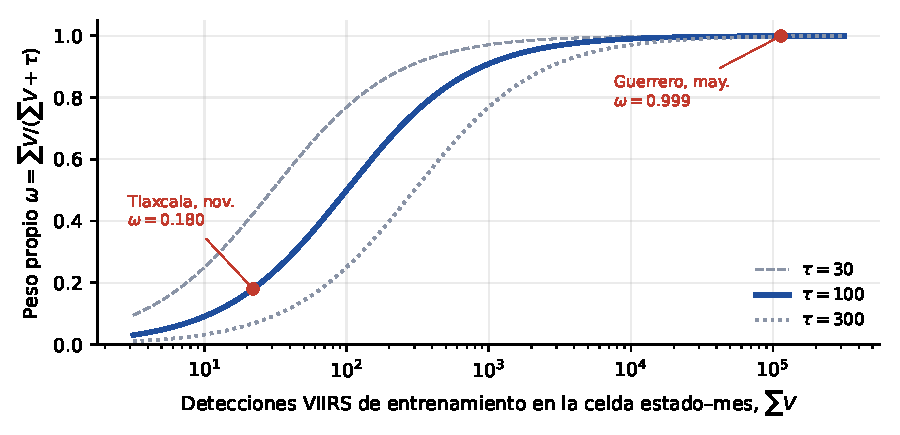
\includegraphics[width=0.85\textwidth]{fig/fig_contraccion.pdf}
\caption{Peso propio $\omega$ de una celda estado--mes según sus detecciones de VIIRS de entrenamiento. Con $\tau=100$, una celda con 22 detecciones (Tlaxcala en noviembre) pone solo $18\,\%$ en su propio dato; una celda con más de cien mil (Guerrero en mayo) pone prácticamente todo.}\label{fig:contraccion}
\end{figure}

\subsection{Ejemplos con datos reales}

\begin{table}[H]
\centering
\caption{Efecto de la contracción en cuatro celdas estado--mes (entrenamiento 2012--2019). $\widehat k$ es la razón de la ecuación~\eqref{eq:khat}; $\widetilde k$, la de la ecuación~\eqref{eq:ktilde}; CV es el piso de la ecuación~\eqref{eq:cv}.}\label{tab:ejemplos}
\small
\begin{tabular}{@{}lrrrrrrr@{}}
\toprule
Celda & $\sum M$ & $\sum V$ & $\widehat k$ & $\widehat k_{\mathrm{nac}}$ & $\omega$ & $\widetilde k$ & CV (\%) \\
\midrule
Tlaxcala (noviembre) & 6 & 22 & 0.273 & 0.251 & 0.180 & 0.255 & 46.1 \\
Aguascalientes (agosto) & 35 & 20 & 1.750 & 0.242 & 0.167 & 0.493 & 28.0 \\
Morelos (octubre) & 5 & 40 & 0.125 & 0.270 & 0.286 & 0.229 & 47.4 \\
Guerrero (mayo) & 26\,402 & 113\,412 & 0.233 & 0.247 & 0.999 & 0.233 & 0.7

\\
\bottomrule
\end{tabular}
\end{table}

En Aguascalientes en agosto, con 20 detecciones de VIIRS y 35 de MODIS, la razón propia ($1.75$) es siete veces el valor nacional ($0.24$): confiar en ella convertiría cada detección de VIIRS en casi dos hotspots equivalentes. La contracción la lleva a $0.49$. En cambio, en Guerrero en mayo el factor casi no se mueve. Esa es la conducta buscada: corregir donde hay ruido y respetar donde hay información.

\section{Elección de \texorpdfstring{$\tau$}{tau}}\label{sec:tau}

El parámetro $\tau$ se probó en la rejilla $\{0,10,30,100,300,1000\}$ con los dos ejercicios de validación del capítulo~\ref{cap:valid}. La tabla~\ref{tab:tau} la reproduce a partir de los CSV publicados.

\begin{table}[H]
\centering
\caption{Error de la calibración por estado y mes según $\tau$. Con $\tau=0$ no hay contracción. Valores en \%.}\label{tab:tau}
\small
\begin{tabular}{@{}rcccc@{}}
\toprule
 & \multicolumn{2}{c}{Error por estado y mes} & \multicolumn{2}{c}{Error anual nacional}\\
\cmidrule(lr){2-3}\cmidrule(lr){4-5}
$\tau$ & Un año fuera & Fuera de muestra & Un año fuera & Fuera de muestra \\
\midrule
0 & 13.0 & 14.9 & 1.2 & 2.6 \\
10 & 12.9 & 14.7 & 1.3 & 2.3 \\
30 & 12.9 & 14.6 & 1.3 & 2.2 \\
\textbf{100} & \textbf{12.9} & \textbf{14.5} & \textbf{1.3} & \textbf{2.1} \\
300 & 12.9 & 14.5 & 1.3 & 2.1 \\
1000 & 13.1 & 14.5 & 1.4 & 2.1

\\
\bottomrule
\end{tabular}
\end{table}

La conclusión es que la superficie de error es plana: entre $\tau=30$ y $\tau=300$ el error por estado y mes cambia en menos de dos décimas de punto porcentual en ambos ejercicios. Quitar toda la contracción ($\tau=0$) cuesta unos $0.4$ puntos porcentuales en el error fuera de muestra, y contraer demasiado ($\tau=1000$) empeora algo el ejercicio de un año fuera.

\begin{cuidado}[Una precisión de honestidad]
Elegimos $\tau=100$ comparando los dos ejercicios, incluido el de 2020--2025. Por eso ese conjunto no es del todo «virgen» para esta decisión. Como el efecto de $\tau$ es de décimas de punto y plano en un rango amplio, el sesgo de selección es pequeño, pero conviene decirlo. Los demás parámetros del capítulo~\ref{cap:pron} se ajustaron con otro criterio: solo con años anteriores a 2020.
\end{cuidado}

\section{Un detalle: enero de 2012}

VIIRS S-NPP empieza el 20 de enero de 2012. Por eso el mes de enero de 2012 está incompleto para VIIRS y se excluye al calibrar y al evaluar: se elimina de $\sum M$ y de $\sum V$ (y de los errores de la validación). Sin esta exclusión, enero tendría un factor artificialmente alto, porque MODIS cuenta el mes completo y VIIRS solo once días.

\begin{ideaclave}[Idea clave del capítulo]
El factor de calibración es una razón de totales, $\widehat k=\sum M/\sum V$, que sale de máxima verosimilitud condicional y no exige modelar la intensidad del fuego de cada año. Su error relativo es del orden de $\sqrt{1/\sum M+1/\sum V}$. Donde hay pocos datos, la contracción con $\tau=100$ lo acerca al valor nacional del mismo mes, y esa corrección equivale a una media a posteriori beta--binomial.
\end{ideaclave}
